\chapter{Residual Neural Networks}
Recall that 
\begin{equation}
f^j = \theta^j \circ g\circ f^{j-1}= \theta^j \circ g\circ
\theta^{j-1} \circ g \circ f^{j-2} 
\end{equation}
\begin{equation}\label{fjj}
f^j = \theta^j \circ g\circ \theta^{j-1} \circ x_{j-1}
\end{equation}
where
\begin{equation}
  \label{eq:4}
x_{j-1}=g \circ f^{j-2}, \quad x_0=x  
\end{equation}
We note \eqref{fjj} can be viewed as a nonlinear encoder for
$x_{j-1}$.  We now introduce the enhanced encoder has follows:
\begin{equation}
  \label{tildefj}
  \tilde f^j=f^{j}+\tilde \theta_{j-1}\circ x_{j-1}
\end{equation}
which is the main idea used for ResNet. 

So we have the network like:
\begin{equation}
\begin{cases}
f^{2j} &= \theta^{2j} \circ g^{2j}( \tilde f^{2j-1}), \\
f^{2j-1} &= \theta^{2j-1} \circ g^{2j-1}(f^{2j-2}), \\
f_0 &= \theta^0(x).
\end{cases} \\
\end{equation}
When $\tilde \theta_{j}$ is a square ``matrix", we can just take $ \theta_{j} = I$, this is what ResNet often used.

Let us make some comments
\begin{enumerate}
\item It has been numerically observed that when $n_j=n_{j-1}$, one can take 
  \begin{equation}
    \label{eq:1}
\theta_j=id.    
  \end{equation}
\item In the usual CNN, it may happen that $\theta^j\approx 0$.  This
  means that the information is getting ``lost'' at the current level
  by ``improper'' (too much?) pooling or stride.  In this case,
  \eqref{tildefj} helps ``recover'' the information from the previous
  layer.   In this case
  \begin{equation}
\tilde f^j\approx x_{j-1}    
  \end{equation}
\item Continuing with the above argument, it is then reasonable to
  expect that ResNet can use very large number of layers so that the
key features are still well kept from layer to layer.
\end{enumerate}

\bigskip 
\bigskip 
\begin{equation}
f^j = \theta^j \circ g^j(f^{j-1} + g\circ f^{j-3}) ),
\end{equation}

Take 
\begin{equation}
x = g\circ f^{j-3},
\end{equation}
so $f^{j-1}$ is a function of $x$ as:
\begin{equation}
f^{j-1} = \theta^{j-1} \circ g \circ \theta^{j-1} (x).
\end{equation}

\section{ResNet model based on classical notation}
For general image classification problems, many numerical results shows that, if we just use the general CNN structure, you will get worse generallization error with deeper network. However, after 2015, Kaiming He and etc found that if they adopt the ``shortcut" structure into the general CNN they will get better result as networks become deeper and deeper in some degree and they call that kinds of CNN model as ResNet. After that, all state-of-art DL models adopt the ResNet properties to construct those deep CNN models with low generalization error. 

\subsection{Shortcut connection and ResNet models}
First, we would like to talk about the so called ``shortcut connection" in general neural network. As we know, the output of $f_j$ is dependent with $f_i$ for all $ i < j$, but is just decided by $f_{j-1}$ directly and this can be shown in BP algorithm. Shortcut connection means to make the direct dependence longer like 
\begin{equation}
f^j = \theta^j \circ g^j \circ h( f^{j-1}, \cdots, f^{j-k}).
\end{equation} 

If we use the idea of encoder for CNN, we can take both $f^j$ with $j = 1:J$ as the nonlinear encoder of data. By the way, we can also think that $f^j$ is the nonlinear encoder of $f^i$ with $i < j$.  So, we may take $h$ as:
\begin{equation}
h(f^{j-1}, \cdots, f^{j-k}) = f^{j-1} + \sum_{s = 2}^k P_{j-s}^{j-1} f^{j-s}.
\end{equation}
or we need to add nonlinear map as:
\begin{equation}
h(f^{j-1}, \cdots, f^{j-k}) = f^{j-1} + \sum_{s = 2}^k P_{j-s}^{j-1} g^{j-s+1}(f^{j-s}).
\end{equation}





So, in fact we have many choice for change ResNet models, now we just introduce what kinds of shortcut connection in  RestNet. 
\begin{equation}
f^j = \theta^j \circ g^j(f^{j-1} + P^jg^{j-2}(f^{j-3}) ),
\end{equation}
this can be shown in the next figure:
\begin{figure}[!htb]
	\center{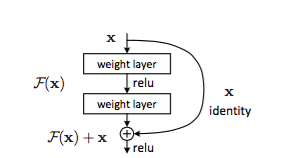
\includegraphics[width=6cm] {figures/ShortCut.png}}        
	\caption{The Architecture of ShortCut Connection with Distance 2}      
	\label{LeNet-5}
\end{figure}
So, a general ResNet structure would be like:
\begin{equation}
\begin{cases}
f^{2j-1} &= \theta^{2j-1} \circ g^{2j-1}(f^{2j-2}), \\
\tilde f^{2j-1} &= f^{2j-1} + g\circ \tilde f^{2(j-1)-1}, \\
f^{2j} &= \theta^{2j} \circ g^{2j}(\tilde f^{j-1}),  \\
f_0 &= \theta^0(x).
\end{cases}
\end{equation}



\subsection{ResNet in ImageNet}
Here is a table to show the general structure for ResNet for ImageNet in 2015.
\begin{figure}[!htb]
	\center{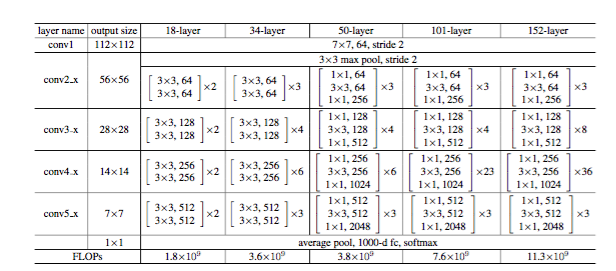
\includegraphics[width=10cm] {figures/ResNet_ImageNet.png}}        
	\caption{The Architecture of RestNet for ImageNet}      
	\label{LeNet-5}
\end{figure}

The $\times 2$ block is the same to above, and the $\times 3$ block is shown next:
Here is a table to show the general structure for ResNet for ImageNet in 2015.
\begin{figure}[!htb]
	\center{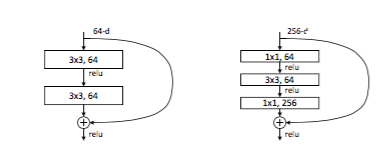
\includegraphics[width=6cm] {figures/ShortCut2.png}}        
	\caption{The Architecture of two kinds of shortcut connection}      
	\label{LeNet-5}
\end{figure}
Or we can show it as:
\begin{equation}
f^j = \theta^j \circ g^j(f^{j-1} + P^jg^{j-3}(f^{j-4}) ),
\end{equation}
then the network would like:
\begin{equation}
\begin{cases}
f^{3j-2} &= \theta^{3j-2} \circ g^{3j-2}(f^{3(j-1)}), \\
f^{3j-1} &= \theta^{3j-2} \circ g^{3j-1}({f}^{3j-2}) \\
\tilde{f}^{3j-1} &= f^{3j-1} + g(\tilde f^{3(j-1)-1}), \\
f^{3j} &= \theta^{3j}\circ g^{3j}(\tilde f^{3j-1}) \\
f_0 &= \theta^0(x).
\end{cases} 
\end{equation}

\subsection{Some properties of ResNet v.s PlainNet}
In the first paper about the ResNet, the authors proposed some properties of ResNet:
\begin{enumerate}
\item In some region, the deeper network the better results for ResNet. But, this cannot hold for plain network generally. 
\begin{figure}[!htb]
	\center{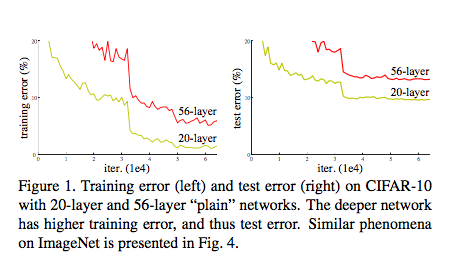
\includegraphics[width=6cm] {figures/PlainNet.png}}        
	\caption{The Architecture of two kinds of shortcut connection}      
	\label{LeNet-5}
\end{figure}

\begin{figure}[!htb]
	\center{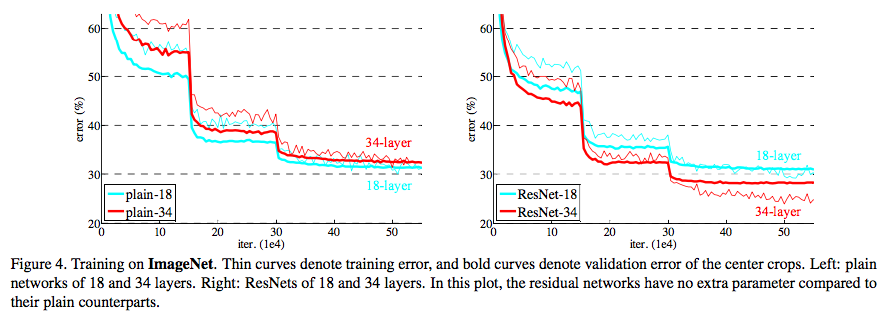
\includegraphics[width=10cm,height=4.5cm] {figures/PlianNetvsResNet.png}}        
	\caption{The Architecture of two kinds of shortcut connection}      
	\label{LeNet-5}
\end{figure}

\begin{figure}[!htb]
	\center{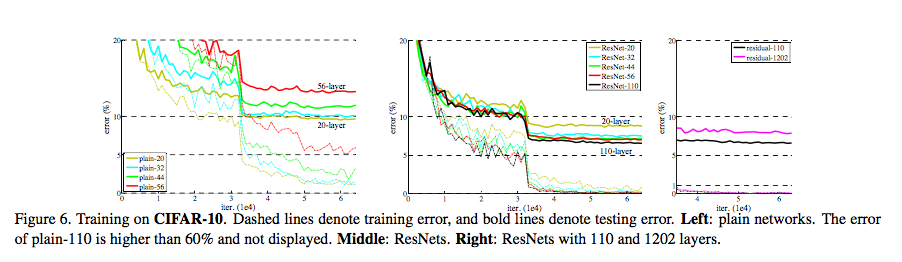
\includegraphics[width=12cm,height=4cm] {figures/PlianNetvsResNet-10.png}}        
	\caption{The Architecture of two kinds of shortcut connection}      
	\label{LeNet-5}
\end{figure}


\item Generally speaking, ResNet networks can be trained more easily than the plain network with the same depth.

\item For some case, if the pooling or convolution with stride is bigger than 1, the size of $f^{j-1}$ and $g^{j-3}(f^{j-4})$ are not the same, so we may need a "interpolation-restriction" matrix $P_{j-3}^{j-1}$ for the essential dimension is restriction but the channel dimension is restriction. And even for the dimension is the same, we can also use a transform for this operator i.e
\begin{equation}
f^j = \theta^j \circ g^j(f^{j-1} + P^jg^{j-2}(f^{j-3}) ),
\end{equation}
In the first paper about the ResNet, there are some numerical results to show that, P is only adopted when the dimension is changed.
\begin{figure}[!htb]
	\center{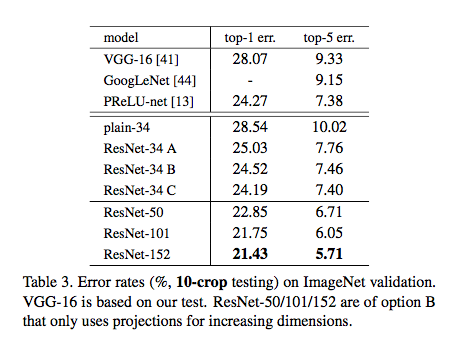
\includegraphics[width=6cm] {figures/ResNetProjection.png}}        
	\caption{The Architecture of two kinds of shortcut connection}      
	\label{LeNet-5}
\end{figure}

For the next three strategies:
\begin{enumerate}
\item Zero-padding shortcuts are used for increasing dimensions, and all shortcuts are parameter-free, i,e all $P^j$ is fix.
\item Projection shortcuts are used for increasing dimensions, and other shortcuts are identity.
\item All shortcuts are projections, i.e we need train all $P^j$.
\end{enumerate}


\section{One developed ResNet model}
For this model, which can be expressed as:
\begin{equation}\label{I_ResNet_old}
	\begin{cases}
		f^{2j-1} &= \theta^{2j-1} \circ g^{2j-1}(f^{2j-2}), \\
		\tilde f^{2j-1} &= f^{2j-1} + g\circ \tilde f^{2(j-1)-1}, \\
		f^{2j} &= \theta^{2j} \circ \tilde f^{j-1},  \\
		f_0 &= \theta^0(x).
	\end{cases}
\end{equation}
This can make sense is because of the fact that, if we take 
\begin{equation}
F(x) = \theta \circ g \circ \theta(x)
\end{equation}
and noted
\begin{equation}
g^{j-2}(f^{j-3}) = x^1,
\end{equation}
then we have
\begin{equation}
x^l = P^lx^{l-1} + F^l(x^{l-1}),
\end{equation}
and for $P^{l} = I$ for almost cases.  For example, $P^l = I$ for $l = t+1: T$, which means:
\begin{equation}
x^T = x^t + \sum_{l=t}^{T} F^l(x^{l-1}).
\end{equation}
which means that information can transform for long distance especially between two pooling operations.

\newpage
\subsection{A look at some special case}
Let us take $j=9$ in \eqref{ResNet0}

\begin{equation}\label{ResNet9}
  \begin{array}{rcl}
f^0&=&\theta^0(x)\\    
f^1&=&\theta^1\circ g\circ f^0(x)\\    
\tilde f^1&=&f^1 \\
f^2&=&\theta^2\circ g\circ f^1(x)\\    
f^3&=&\theta^3\circ g\circ f^2(x)\\    
\tilde f^3&=&f^3+g\circ \tilde f^1 \\
f^4&=& \theta^4\circ g\circ \tilde f^3(x) \\
f^5&=&\theta^5\circ g\circ f^4(x)\\    
\tilde f^5&=&f^5+g\circ \tilde f^3 \\
f^6&=&\theta^6\circ g\circ \tilde f^5(x)\\    
f^7&=&\theta^7\circ g\circ f^6(x)\\  
\tilde f^7&=&f^7+g\circ \tilde f^5 \\
 f^8&=& \theta^8\circ g\circ\tilde f^7(x) \\ 
 f^9&=& \theta^9 \circ g \circ f^8(x)
  \end{array}
\end{equation}

The above equation \eqref{ResNet9} shows the ResNet with 9 layers and step-2.

Now if we note
\begin{equation}
y^l = g \circ \tilde{f}^l,
\end{equation}
and
\begin{equation}
F^l(y^l) = \theta^{l+2} \circ g \circ \theta^{l+1}(y^l),
\end{equation}

So the above net work is:
\begin{equation}\label{ResNet9-1}
  \begin{array}{rcl}
f^9 &=& F^7(y^7) \\
y^7 &=& g \circ  [ F^5(y^5) + y^5 ]\\
y^5 &=& g \circ  [F^3(y^3) + y^3 ]\\
y^3 &=& g \circ  [F^1(y^1) + y^1 ]\\
y^1 &=& g \circ f^1
  \end{array}
\end{equation}
So, remove the $g$ in \eqref{ResNet9-1} seems very natural in the
above notation.

The most recent 
\begin{equation}\label{ResNet9-1}
  \begin{array}{rcl}
f^9 &=& F^7(y^7) \\
y^7 &=& F^5(y^5) + y^5 \\
y^5 &=& F^3(y^3) + y^3 \\
y^3 &=& F^1(y^1) + y^1 \\
y^1 &=&  f^1
  \end{array}
\end{equation}
The most recent 
\begin{equation}\label{ResNet9-new}
  \begin{array}{rcl}
f^9 &=& F^7(y^7) \\
y^7 &=& F^5(y^5) + y^5 \\
y^5 &=& F^3(y^3) + y^3 \\
y^3 &=& F^1(y^1) +  y^1 \\
y^1 &=&  f^1
  \end{array}
\end{equation} 
Now adding all the formulas in \eqref{ResNet9-new}, we get
\begin{equation}\label{ResNet9-additive}
f^9 = F^7(y^7) + F^5(y^5) + F^3(y^3) +  F^1(y^1) + f^1
\end{equation}

Recall in multigrid
$$
I-B_kA_kP_k=(I-T_k)(I-B_{k-1}A_{k-1}P_{k-1})
=I-T_k(I-B_{k-1}A_{k-1}P_{k-1})-B_{k-1}A_{k-1}P_{k-1}
$$
$$
B_kA_kP_k=B_{k-1}A_{k-1}P_{k-1}
+T_k(I-B_{k-1}A_{k-1}P_{k-1}) 
$$
$$
B_JA_J=P_1+\sum_{k=2}^JT_k(I-B_{k-1}A_{k-1}P_{k-1}) 
=P_1+\sum_{k=2}^JT_k\prod_{j=1}^{k-1}(I-T_j)
$$

We note that
$$
F^1(y^1)=\theta^3\circ g\circ \theta^2\circ y^1
$$
We can take 
$$
\theta^2=\check \theta^2\circ (I-\hat\theta^1)
$$
We can find 
$$
\bar\theta^3\circ g\circ \bar\theta^2 = I
$$
which means
$$
\sum_{i=1}^k a_ig(w_ix+b_i)+c =x
$$
Now we make some special choices:
\begin{equation}\label{id}
\bar\theta^3\circ g\circ (\bar\theta^2\circ(\theta^2-I)) = \theta^2-I
\end{equation}
Thus
$$
y^3=\theta^2\circ y^1
$$
This recovers the linear model! Here to recover the \eqref{id} we only need the have that 

\begin{equation}\label{id_cond}
\theta^3 \in \mathbb{R}^{n\times 2n} \quad \text{and} \quad \theta^2 \in \mathbb{R}^{2n \times n}.
\end{equation}

\newpage

The introduction of the original paper on ResNet \cite{HeKaiming2015} include the following statement:
\begin{quote}\it
  We can also use a square matrix $W_s$ in Eqn. (1). But we will show by experiments that the identity mapping is sufficient for addressing the degradation problem and is economical, and thus $W_s$ is only used when matching dimensions. 
\end{quote}
In our notation, $W_s$ is just the $\tilde\theta^3$ in \eqref{ResNet4}.

We now compare a usual DNN as follows
\begin{equation}\label{OriginalResNet4}
  \begin{array}{rcl}
f^0&=&\theta^0(x)\\    
f^1&=&\theta^1\circ g\circ f^0(x)\\    
&\vdots& \\        
f^9&=&\theta^9\circ g\circ f^8(x)
  \end{array}
\end{equation}
\end{enumerate}

We now study the relationship between \eqref{ResNet4} and \eqref{OriginalResNet4}.  Our question is then: Can we find weights such that the following identity holds
\begin{equation}
\label{ResNet4}
\theta^4\circ g\circ f^3=\tilde \theta^4\circ g\circ[f^3+\tilde \theta^3\circ g\circ f^1].    
\end{equation}
and furthermore $\tilde \theta^3$ is non-singular? 

Let us first consider the case that $g=id$, we ask
$$
\theta^4\circ f^3=\tilde \theta^4[f^3+\tilde \theta^3\circ f^1].    
$$
$$
\theta^4\circ \theta^3\circ \theta^2 f^1=\tilde \theta^4[\theta^3\circ \theta^2 f^1+\tilde \theta^3\circ f^1].    
$$
$$
\theta^4\circ \theta^3\circ \theta^2 =\tilde \theta^4\circ [\theta^3\circ \theta^2 +\tilde \theta^3].    
$$


\newpage
\subsection{New notation}
\begin{equation}
  \label{extractor}
H_k(x)=\xi^k\circ g\circ \eta_k(x)  
\end{equation}
The ResNet can then be written as
\begin{equation}  \label{RNk}
x^k=x^{k-1}+H_k(x^{k-1}), \quad k=1:J  
\end{equation}
with 
$$
x^0=x.
$$
We make the following observations:
\begin{enumerate}
\item \eqref{RNk} looks like nonlinear ``smoother'' or ``rougher'',
  but it is a combination of additive-multiplicative or
  BPX like.  It is like Block Gauss-Seidel with each block given by Jacobi.
\item We can make the above procedure to be multiplicative, which may
  improve efficiency. 
\item Each different $k$ in \eqref{RNk} gives a new layer in the
  ResNet, but these are kind of ``fake'' layers.
\item The really new layer is only created by restriction, such as
  ``stride''
\item Different $H_k$ gives more parameters, which in a way gets
  closer to the variable convolution ... which corresponds to
  \begin{enumerate}
\item more different kernels on each pixel point
\item  more channels, 
\end{enumerate}
\item The real layers should only be given when the dimension of the 
  problem changes.   Namely the dimensions of different layers has to be
  different. 
\item The relationship between ResNet and PlainNet is as follows:
  \begin{enumerate}
  \item PlainNet is Gauss-Seidel
\item ResNet is to convert part of the above Gauss-Seidel by a mixture
  of   Gauss-Seidal and Jacobi!
  \end{enumerate}
\end{enumerate}

\subsubsection{New terminology: ``extractor''}
We call each $H_k$ as 
\begin{enumerate}
\item ``extractor''
\item smoother
\item rougher
\end{enumerate}



